\documentclass[t,dvipsnames,hyperref={colorlinks,citecolor=NavyBlue,linkcolor=NavyBlue,anchorcolor=NavyBlue,urlcolor=NavyBlue}]{beamer}

\setbeamertemplate{navigation symbols}{}
\useinnertheme{circles}
% \usecolortheme{crane}

% \usepackage[T1]{fontenc}
\usepackage[utf8]{inputenc}
% \usepackage[polish]{babel}
\usepackage[british]{babel}

\usepackage[adobe-utopia]{mathdesign}
\usepackage[series=z]{libgreek}
\usepackage{tgpagella}
\usepackage[textwidth=4cm]{todonotes}
\usepackage{minted}
\usemintedstyle{colorful}
\usepackage{enumitem}
% \usemintedstyle{autumn}
% \usemintedstyle{vs}
\usepackage{tikz}
\usetikzlibrary{matrix,arrows,calc}
\tikzset{every scope/.style={>=angle 60,thick}}

\author{Marcin Szamotulski}
\institute{\insertlogo{
\includegraphics[height=1cm]{iohk-logo.png}}}
\title{Monoidal Synchronisation}
\subtitle{\small case study on \href{https://github.com/input-output-hk/ouroboros-network}{ouroboros-network}}

\setbeamertemplate{frametitle}[default][center]

\begin{document}
\begin{frame}
    \titlepage
\end{frame}

\part{Introduction}
\begin{frame}
  \partpage
  \tableofcontents[part=1]
\end{frame}

%%%%%%%%%%%%%%%%%%%%
\section{Semigroups}
%%%%%%%%%%%%%%%%%%%%

\begin{frame}[fragile]
  \frametitle{Semigroups}
  \begin{minted}[stripall,bgcolor=NavyBlue!5!white,fontsize=\small]{haskell}
class Semigroup a where
  -- associativity: (a <> b) <> c == a <> (b <> c)
  (<>) :: a -> a -> a
  \end{minted}

  \begin{examples}\small
    \begin{minted}[stripall,bgcolor=NavyBlue!5!white,fontsize=\small]{haskell}
-- free semigroup with one generator
instance Semigroup (NonEmpty a) where
  (a :| as) <> (b :| bs) = a :| as ++ b : bs

instance Semigroup [a] where
  (<>) = (++)

instance Semigroup a => Semigroup (Maybe a) where
  Nothing <> a = a
  a <> Nothing = a
  Just a  <> Just b = Just (a <> b)
    \end{minted}
  \end{examples}
\end{frame}

\begin{frame}[fragile]
  \frametitle{Foldable1 type class}
  \vspace{-4mm}
  \begin{minted}[stripall,bgcolor=NavyBlue!5!white,fontsize=\small]{haskell}
-- from "semigroupoids" package
class Foldable t => Foldable1 t where
  foldMap1 :: Semigroup m
           => (a -> m) -> t a -> m
  fold1 :: Semigroup m => t m -> m
  fold1 = foldMap1 id
  toNonEmpty :: t a -> NonEmpty a
  toNonEmpty = foldMap1 (:| [])
  \end{minted}
  \vspace{-5mm}
  \begin{examples}\footnotesize
    The canonical example instance is \texttt{NonEmpty}; all the instances
    require that the container is non-empty
    \footnote{This is a consequence of a \texttt{Semigroup} constraint rather
    than the \texttt{toNonEmpty} class
    member.}.
    \vspace{-2mm}
    \begin{minted}[stripall,bgcolor=NavyBlue!5!white,fontsize=\small]{haskell}
instance Foldable1 NonEmpty where
  -- proof that @NonEmpty@ is a free semigroup:
  foldMap1 :: Semigroup m => (a -> m) -> NonEmpty a -> m
  foldMap1 f (a :| (b : bs)) = f a <> foldMap1 f (b :| bs)
  foldMap1 f (a :| [])       = f a
    \end{minted}
  \end{examples}
\end{frame}

%%%%%%%%%%%%%%%%%
\section{Monoids}
%%%%%%%%%%%%%%%%%

\begin{frame}[fragile]
  \frametitle{Monoids}
  \begin{minted}[stripall,bgcolor=NavyBlue!5!white,fontsize=\small]{haskell}
class Semigroup a => Monoid a where
  -- two sided identity
  -- > a <> mempty == a == mempty <> a
  mempty :: a
  \end{minted}

  \vspace{-2mm}
  \begin{examples}\small
    \vspace{-2mm}
    \begin{minted}[stripall,bgcolor=NavyBlue!5!white,fontsize=\small,mathescape]{haskell}
-- free monoid in the class of left-strict monoids
instance Monoid [a] where
  mempty = []

-- left adjoint to the forgetful functor from monoids
-- to semigroups, i.e. `Maybe s $\rightarrow_{monoid}$ m $\equiv$ s $\rightarrow_{semigroup}$ m`
instance Semigroup a => Semigroup (Maybe a) where
  Nothing <> a       = a
  a       <> Nothing = a
  Just a  <> Just b  = Just (a <> b)
instance Semigroup a => Monoid (Maybe a) where
  mempty = Nothing
    \end{minted}
  \end{examples}
\end{frame}

\begin{frame}[fragile]
  \frametitle{Foldable type class}
  \begin{minted}[stripall,bgcolor=NavyBlue!5!white,fontsize=\small]{haskell}
class Foldable t where
  foldMap :: Monoid m => (a -> m) -> t a -> m
  fold :: Monoid m => t m -> m
  fold = foldMap id
  toList :: t a -> [a]
  toList = foldMap (\a -> [a]) 
  \end{minted}

  Advantage of \texttt{foldMap} over \texttt{foldr}:
  \begin{minted}[stripall,bgcolor=NavyBlue!5!white,fontsize=\small]{haskell}
foldMap :: (Foldable t, Monoid m)
        => (a -> m) -> t a -> m
foldMap f = foldr (\a m -> f a <> m) mempty
  \end{minted}
\end{frame}

%%%%%%%%%%%%%%%%%%%%%%
\section{FreeAlgebras}
%%%%%%%%%%%%%%%%%%%%%%

\begin{frame}[fragile]
  \frametitle{Free algebras}
  {\small
    The \texttt{FreeAlgebra} type class can capture the heart of \texttt{Foldable} and
    \texttt{Foldable1} classes and can be defined for other algebras than
     semigroups (\texttt{Foldable1}) or monoids (\texttt{Foldable}).
  }
  \begin{minted}[stripall,bgcolor=NavyBlue!5!white,fontsize=\small]{haskell}
class FreeAlgebra (m :: Type -> Type) where
  returnFree  :: a -> m a
  foldMapFree :: forall d a. AlgebraType  m d
              => (a -> d) -> m a -> d
  \end{minted}
  {\small
  For more details see
  \begin{itemize}
    \item[\bullet] \href{https://skillsmatter.com/skillscasts/13007-lightning-talk-rethinking-freeness-through-universal-algebra}{Haskell eXchange lightning talk},
    \item[\bullet] \href{https://hackage.haskell.org/package/free-algebras}{free-algebras}
      package on Hackage.
  \end{itemize}
  }
\end{frame}

\section{Near Semi-Rings}
\begin{frame}
  \frametitle{Near Semi-Ring}
  \begin{definition}
    \((S, +, \cdot, 0)\) is a near semi-ring if:
    \begin{itemize}
      \item[\bullet] \((S, +, 0)\) is a monoid (not necessarily abelian);
      \item[\bullet] \((S, \cdot)\) is a semigroup;
      \item[\bullet] \((a + b) \cdot c = a \cdot c + b \cdot c\);
      \item[\bullet] \(0 \cdot a = 0\).
    \end{itemize}
  \end{definition}
  \begin{example}\small
    if \(M\) is a monoid then all its monoid homomorphisms form a near semi-ring
    with:
    \begin{itemize}
      \item[\bullet] \textit{multiplication}: function composition
      \item[\bullet] \textit{addition}: pointwise addition
      \item[\bullet] \textit{zero}: constant function to the identity of the monoid.
    \end{itemize}
    Note that for this \textit{near semi-ring} we have \(0\cdot a = 0 = a \cdot 0\),
    since monoid homomorphisms preserve the identity element.
  \end{example}
\end{frame}

%%%%%%%%%%%%%%%%%%%%%%%%%%%%%%%%%%%%%%%%%%%%
\section{First-to-Finish and Last-to-Finish}
%%%%%%%%%%%%%%%%%%%%%%%%%%%%%%%%%%%%%%%%%%%%

\begin{frame}[fragile]
  \frametitle{First-to-Finish}
  Multiplicative semigroup of the \text{LastToFinish}, \texttt{FirstToFinish} near semi-ring.
  \begin{minted}[stripall,bgcolor=NavyBlue!5!white,fontsize=\small]{haskell}
newtype FirstToFinish m a =
        FirstToFinish { runFirstToFinish :: m a }
  deriving ( Generic,     Generic1
           , Applicative, Alternative
           , Monad,       MonadPlus
           , Functor,     Traversable
           )
  deriving Semigroup     via (Alt m a)
  deriving Monoid        via (Alt m a)
  deriving Foldable      via (Alt m)
  deriving Contravariant via (Alt m)

(<|>) :: Alternative m
      => m a -> m a -> m a

% This works well for `IO` and `STM`!
  \end{minted}
\end{frame}

\begin{frame}[fragile]
  \frametitle{Last-to-Finish}
  Additive semigroup of the \text{LastToFinish}, \texttt{FirstToFinish} near semi-ring.
  \begin{minted}[stripall,bgcolor=NavyBlue!5!white,fontsize=\small]{haskell}
newtype LastToFinish m a =
        LastToFinish { runLastToFinish :: m a }
  deriving ( Generic,     Generic1
           , Applicative, Alternative
           , Monad,       MonadPlus
           , Functor,     Traversable
           )
  deriving Foldable via (Ap m)

instance MonadPlus m => Semigroup (LastToFinish m a) where
    LastToFinish left <> LastToFinish right =
      LastToFinish $ do
        a <-  Left  <$> left
          <|> Right <$> right
        case a of
          Left  {} -> right
          Right {} -> left
  \end{minted}

% This works well for `IO` and `STM`!
\end{frame}

\begin{frame}[fragile]
  \frametitle{Monoidal Last-to-Finish}
  Additive semigroup of the \text{LastToFinishM}, \texttt{FirstToFinish} near semi-ring.
  \begin{minted}[stripall,bgcolor=NavyBlue!5!white,fontsize=\small]{haskell}
newtype LastToFinishM m a =
        LastToFinishM { runLastToFinishM :: m a }
  deriving ( Generic,      Generic1
           , Applicative,  Alternative
           , Monad,        MonadPlus
           , Functor,      Traversable
           )
  deriving Semigroup via (Ap m a)
  deriving Monoid    via (Ap m a)
  deriving Foldable  via (Ap m)

(<+>) :: (Applicative m, Semigroup a)
      => m a -> m a -> m a
(<+>) ma mb = (<>) <$> ma <*> mb

% This works well for `IO` and `STM`!
  \end{minted}


\end{frame}

\part{Case study}
\frame{
  \partpage
  \tableofcontents[part=2]
}

%%%%%%%%%%%%%%%%%%%%%%%%
\section{Ouroboros Network}
%%%%%%%%%%%%%%%%%%%%%%%%

\begin{frame}
  \frametitle{Ouroboros Network}
  \begin{center}
  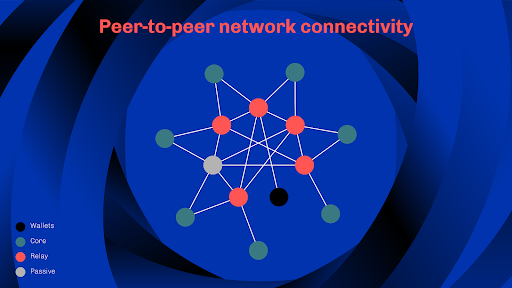
\includegraphics[width=6cm]{../images/p2p-network.png}
  \end{center}
  \begin{itemize}
    \item[\bullet] decentralisad, real-time system
    \item[\bullet] blockchain consensus algorithm based on academic research
    \item[\bullet] core (block producing nodes), relay and end-user nodes all running
      the same core software
  \end{itemize}
\end{frame}

\begin{frame}
  \frametitle{Network Protocol}
  \begin{center}
  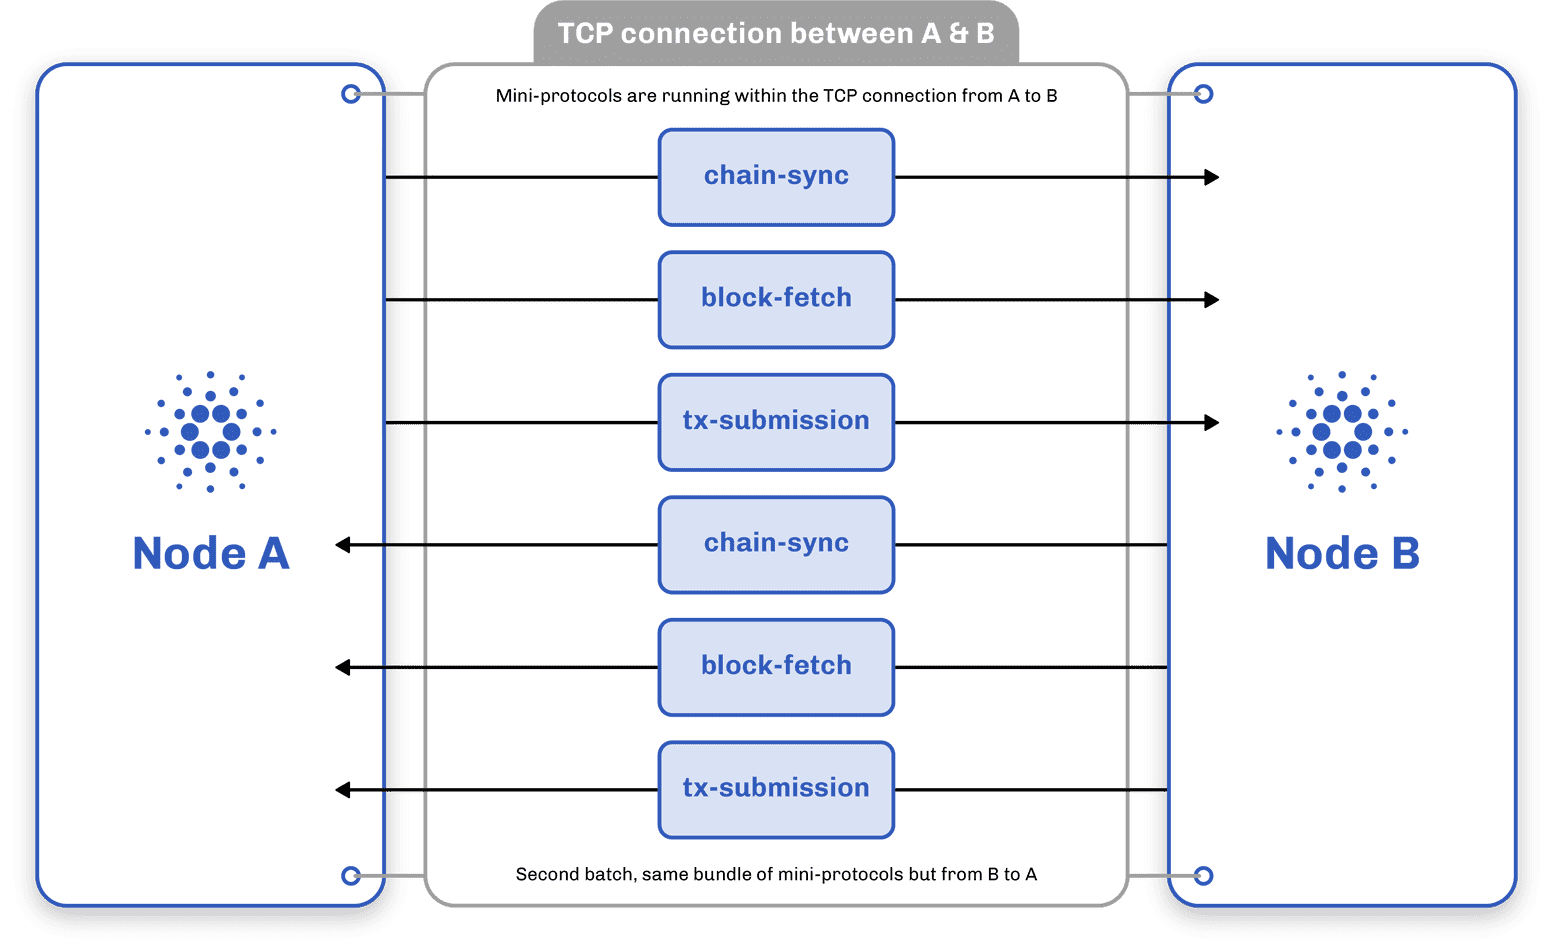
\includegraphics[width=6cm]{../images/node-to-node-ipc.png}
  % TODO: add keep-alive!
  \end{center}
  \begin{itemize}
    \item[\bullet] each node communicates through four mini-protocols:
      \textit{chain-sync}, \textit{block-fetch}, \textit{tx-submission}, \textit{keep-alive};
    \item[\bullet] the mini-protocols are multiplexed over a single bearer;
    \item[\bullet] we use duplex bearers, which means that on each bearer we
      run 8 mini-protocols: inbound (responders) and outbound (initiators).
  \end{itemize}
\end{frame}

%%%%%%%%%%%%%%%%%%%%%
\section{Multiplexer}
%%%%%%%%%%%%%%%%%%%%%

\begin{frame}
  \frametitle{Multiplexer}
  \vspace{-5mm}\small
  \begin{center}
  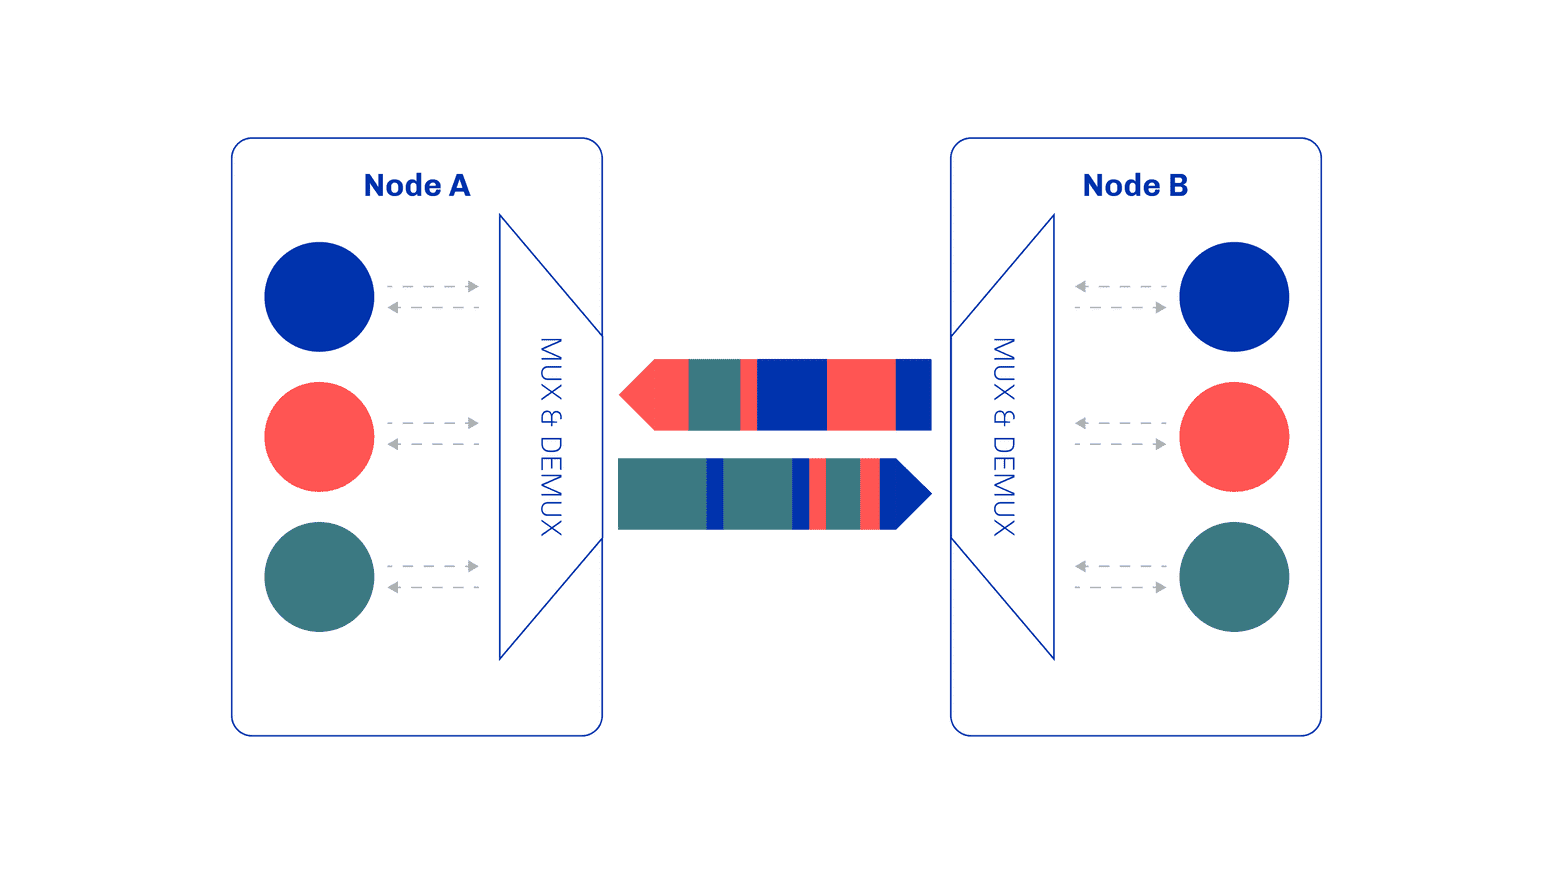
\includegraphics[width=8cm]{../images/multiplexer.png}
  \end{center}
  \vspace{-5mm}
  \begin{itemize}
    \item[\bullet] exectue a set (mini-)protocols on a single bearer (e.g. \texttt{TCP} connection, unix pipe, etc);
    \item[\bullet] bidirectional: allows to run two copies of the protocols: inbound (responder) / outbound (initiator);
    \item[\bullet] no ahead of line blocking;
    \item[\bullet] allows to start responders either \textit{eagerly} or \textit{on
      demand}, e.g. as soon as data arrives for that protocol;
    \item[\bullet] allows to track state of each mini-protocol using \texttt{STM}:
      whether an \textit{on demand} started protocol started running, or if it finished
      / errored.
  \end{itemize}
\end{frame}

\begin{frame}[fragile]
  \frametitle{Multiplexer}
  \begin{minted}[stripall,bgcolor=NavyBlue!5!white,fontsize=\tiny]{haskell}
monitor :: forall mode.
        => Tracer IO MuxTrace
        -> TimeoutFn IO
        -> JobPool.JobPool MuxGroup IO MuxJobResult
        -> EgressQueue IO
        -> TQueue IO (ControlCmd mode IO)
        -> StrictTVar IO MuxStatus
        -> IO ()
monitor tracer timeout jobpool egressQueue cmdQueue muxStatus =
    go (MonitorCtx Map.empty)
  where
    go :: MonitorCtx m mode -> m ()
    go !monitorCtx@MonitorCtx { mcOnDemandProtocols } = do
      result <- atomically $ runFirstToFinish $
            -- wait for a mini-protocol thread to terminate
           (FirstToFinish $ EventJobResult <$> JobPool.collect jobpool)

            -- wait for a new control command
        <> (FirstToFinish $ EventControlCmd <$> readTQueue cmdQueue)

            -- or wait for data to arrive on the channels that do not yet have
            -- responder threads running
        <> foldMap
             (\(ptclState, ptclAction) ->
               FirstToFinish $ do
                 checkNonEmptyQueue (miniProtocolIngressQueue ptclState)
                 return (EventStartOnDemand ptclState ptclAction)
             )
             mcOnDemandProtocols

      case result of
        ...
  \end{minted}
\end{frame}

%%%%%%%%%%%%%%%%%%%%%%%%%%%%%%%%%%%
\section{Inbound Protocol Governor}
%%%%%%%%%%%%%%%%%%%%%%%%%%%%%%%%%%%

\begin{frame}[fragile]
  \frametitle{Inbound Protocol Governor}
  % TODO: I need graphics which shows architecture of all the components, this
  % will make things easier to read.
  \tiny
  \begin{itemize}
    \item[\bullet] track state of multiple connections,
    \item[\bullet] thrack state of each responder mini-protocol.
  \end{itemize}
  \begin{minted}[stripall,bgcolor=NavyBlue!5!white,fontsize=\tiny]{haskell}
data InboundGovernorState muxMode peerAddr a b =
    InboundGovernorState {
        -- | Map of connections state.  Modifying 'igsConnections' outside of
        -- 'inboundGovernorLoop' is not safe.
        --
        igsConnections   :: !(Map (ConnectionId peerAddr)
                                  (ConnectionState muxMode peerAddr a b)),
        ...
      }

data ConnectionState muxMode peerAddr a b = ConnectionState {
      -- | Multiplexer interface for the connection.
      --
      csMux             :: !(Mux.Mux muxMode),

      -- | Static data which describes all mini-protocols supported by the
      -- connection.
      --
      csMiniProtocolMap :: !(Map MiniProtocolNum
                                 (MiniProtocolData muxMode a b)),

      -- | Map of all running mini-protocol completion STM actions.
      --
      csCompletionMap   :: !(Map MiniProtocolNum
                                 (STM (Either SomeException b))),

      ...
    }
  \end{minted}
\end{frame}

\begin{frame}[fragile]
  \begin{minted}[stripall,bgcolor=NavyBlue!5!white,fontsize=\tiny]{haskell}
firstConnectionToFinish InboundGovernorState muxMode peerAddr IO a b
              -> STM (ConnectionId peerAddr, Maybe SomeException)
firstConnectionToFinish InboundGovernorState { igsConnections } =
      runFirstToFinish
    . Map.foldMapWithKey
        (\connId ConnectionState { csMux } ->
          FirstToFinish $ (connId,) <$> (Mux.muxStopped csMux :: STM (Maybe SomeException))
        )
    $ igsConnections
  \end{minted}

  \begin{minted}[stripall,bgcolor=NavyBlue!5!white,fontsize=\tiny]{haskell}
firstMiniProtocolToFinish
       InboundGovernorState muxMode peerAddr a b
    -> STM (Terminated muxMode peerAddr a b)
firstMiniProtocolToFinish InboundGovernorState { igsConnections } = runFirstToFinish $
    Map.foldMapWithKey
      (\connId ConnectionState { csMux, csMiniProtocolMap, csCompletionMap } ->
        Map.foldMapWithKey
          (\miniProtocolNum completionAction ->
                (\tResult -> Terminated {
                      tConnId           = connId,
                      tMux              = csMux,
                      tMiniProtocolData = csMiniProtocolMap Map.! miniProtocolNum,
                      tResult
                    }
                )
            <$> FirstToFinish completionAction
          )
          csCompletionMap
      )
      igsConnections
  \end{minted}
\end{frame}

\begin{frame}[fragile]
  \begin{minted}[stripall,bgcolor=NavyBlue!5!white,fontsize=\tiny]{haskell}
firstPeerDemotedToCold
    :: MonadSTM m
    => InboundGovernorState muxMode peerAddr m a b
    -> STM m (Event muxMode peerAddr m a b)
firstPeerDemotedToCold InboundGovernorState { igsConnections } = runFirstToFinish $
    Map.foldMapWithKey
      (\connId
        ConnectionState {
          csMux,
          csRemoteState
        } ->
        case csRemoteState of
          RemoteEstablished ->
                fmap (const (WaitIdleRemote connId))
              . lastToFirstM
              $ (Map.foldMapWithKey
                  (\(_, miniProtocolDir) miniProtocolStatus ->
                    case miniProtocolDir of
                      InitiatorDir -> mempty

                      ResponderDir ->
                        LastToFinishM $ do
                          miniProtocolStatus >>= \case
                            StatusIdle          -> return ()
                            StatusStartOnDemand -> return ()
                            StatusRunning       -> retry
                  )
                  (Mux.miniProtocolStateMap csMux
                     :: Map (MiniProtocolNum, MiniProtocolDir)
                            (STM m MiniProtocolStatus)
                  )
                )
          ...
      )
      igsConnections
  \end{minted}
\end{frame}

%%%%%%%%%%%%%%%%%%%%%%%%%%%%%%%%%%%%
\section{Outbound Protocol Governor}
%%%%%%%%%%%%%%%%%%%%%%%%%%%%%%%%%%%%

\begin{frame}
  \frametitle{Outbound Protocol Governor}
  \begin{itemize}
    \item[\bullet] governs outbound side of a connection (initiator mini-protocols)
    \item[\bullet] An upstream peer might be in one the three states: \textit{hot}, \textit{warm}, \textit{cold}:
      \begin{description}[labelwidth=2em]%[align=parleft,labelsep=5mm]
        \item[\textit{cold}:] a known peer, no outbound mini-protocols are running;
        \item[\textit{warm}:] warm \& established outbound mini-protocols are
          running (\textit{keep-alive} mini-protocol);
        \item[\textit{hot}:]  hot \& established outbound
          mini-protocols are running (\textit{chain-sync}, \textit{block-fetch},
          \textit{tx-submission}, \textit{keep-alive});
      \end{description}
    \item[\bullet] peer discovery (through a future \textit{gossip}
      mini-protocol), currently only relays registered on chain are discoverable;
    \item[\bullet] it is reponsible for sutaining targets of cold, warm \& hot
      peers.
  \end{itemize}
\end{frame}

\begin{frame}[fragile]
  \begin{minted}[stripall,bgcolor=NavyBlue!5!white,fontsize=\tiny]{haskell}
-- | The governor is using @Guarded m (Decision m peeraddr peerconn)@ where 'm'
-- is an 'STM' monad, to drive its progress.
--
data Guarded stm a =
    -- | 'GuardedSkip' is used to instruct that there is no action to be made
    -- by the governor.
    --
    GuardedSkip !(Maybe (Min Time))

    -- | 'Guarded' is used to provide an action through 'FirstToFinish'
    -- synchronisation, possibly with a timeout, to
    -- the governor main loop.
    --
  | Guarded'   !(Maybe (Min Time)) (FirstToFinish stm a)


-- | 'Guarded' constructor which provides an action, possibly with a timeout,
-- to the governor main loop.  It hides the use of 'FirstToFinish'
-- synchronisation.
--
pattern Guarded :: Maybe (Min Time) -> stm a -> Guarded stm a
pattern Guarded a b <- Guarded' a (FirstToFinish b)
  where
    Guarded a b = Guarded' a (FirstToFinish b)

{-# COMPLETE GuardedSkip, Guarded #-}

  \end{minted}
\end{frame}

\begin{frame}[fragile]
  \frametitle{Guarded semigroup}
  \begin{minted}[stripall,bgcolor=NavyBlue!5!white,fontsize=\tiny]{haskell}
-- | 'Guarded' constructor is absorbing in the sense that
--
-- > Guarded x y <> a = Guarded x' y'
-- > a <> Guarded x y = Guarded x' y'
--
-- In the algebraic sense, @'Guarded' (Just minBound) (return x)@ is a left
-- absorbing element when "stm ~ STM m'@ for some monad @m'@.  There is no right
-- absorbing element since there is no right absorbing elemnt in @STM m'@.
--
-- Ref. [absorbing element](https://en.wikipedia.org/wiki/Absorbing_element)
--
instance Alternative stm => Semigroup (Guarded stm a) where
  Guarded'    ta a <> Guarded'    tb b = Guarded'    (ta <> tb) (a <> b)
  Guarded'    ta a <> GuardedSkip tb   = Guarded'    (ta <> tb)  a
  GuardedSkip ta   <> Guarded'    tb b = Guarded'    (ta <> tb)  b
  GuardedSkip ta   <> GuardedSkip tb   = GuardedSkip (ta <> tb)
  \end{minted}
\end{frame}

\begin{frame}[fragile]
  \frametitle{Guarded decisions}
  \begin{minted}[stripall,bgcolor=NavyBlue!5!white,fontsize=\tiny]{haskell}
guardedDecisions :: Time
                 -> PeerSelectionState peeraddr peerconn
                 -> Guarded (STM m) (TimedDecision m peeraddr peerconn)
guardedDecisions blockedAt st =
  -- All the alternative non-blocking internal decisions.
     RootPeers.belowTarget        actions blockedAt  st
  <> KnownPeers.belowTarget       actions     policy st
  <> KnownPeers.aboveTarget                   policy st
  <> EstablishedPeers.belowTarget actions     policy st
  <> EstablishedPeers.aboveTarget actions     policy st
  <> ActivePeers.belowTarget      actions     policy st
  ...

evalGuardedDecisions :: Time
                     -> PeerSelectionState peeraddr peerconn
                     -> m (TimedDecision m peeraddr peerconn)
evalGuardedDecisions blockedAt st =
  case guardedDecisions blockedAt st of
    GuardedSkip _ ->
      -- impossible since guardedDecisions always has something to wait for
      error "peerSelectionGovernorLoop: impossible: nothing to do"
    Guarded Nothing decisionAction -> do
      traceWith debugTracer (TraceGovernorState blockedAt Nothing st)
      atomically decisionAction
    Guarded (Just (Min wakeupAt)) decisionAction -> do
      let wakeupIn = diffTime wakeupAt blockedAt
      traceWith debugTracer (TraceGovernorState blockedAt (Just wakeupIn) st)
      wakupTimeout <- newTimeout wakeupIn
      let wakeup = awaitTimeout wakupTimeout >> pure (wakeupDecision st)
      timedDecision <- atomically (decisionAction <|> wakeup)
      cancelTimeout wakupTimeout
      return timedDecision
  \end{minted}
  % <> ActivePeers.aboveTarget      actions     policy st

  % -- All the alternative potentially-blocking decisions.
  % <> Monitor.targetPeers          actions st
  % <> Monitor.localRoots           actions st
  % <> Monitor.jobs                 jobPool st
  % <> Monitor.connections          actions st
\end{frame}


\begin{frame}
  \frametitle{Acknowledgement}
  \vspace{1cm}
  \begin{itemize}
    \item Duncan Coutts, \href{https://well-typed.com}{Well-Typed}
    \item Neil Davids, \href{http://pnsol.com}{PNSol}
    \item Karl Knuttson, \href{https://iohk.io}{IOHK}
    \item Peter Thompson, \href{http://pnsol.com}{PNSol}
    \item Armando Santos, \href{https://well-typed.com}{Well-Typed}
  \end{itemize}
\end{frame}
\end{document}
